\documentclass[border=1pt]{standalone}
\usepackage{tikz}
\usetikzlibrary{calc}
\usepackage{mwe}
\begin{document}
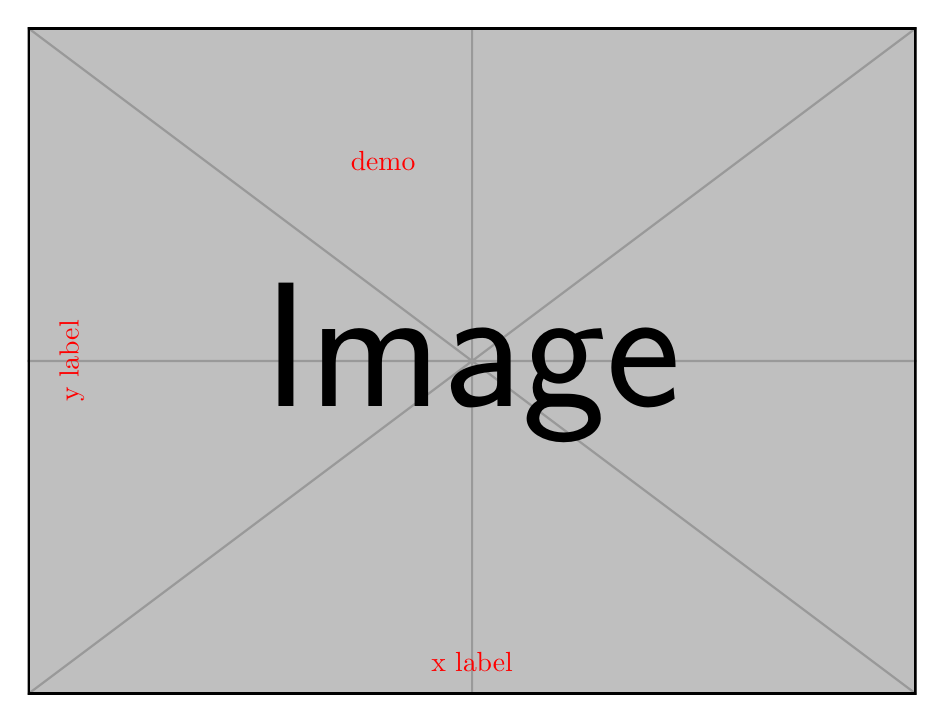
\begin{tikzpicture}
  \node[inner sep=0pt] (A) {\includegraphics{example-image}};
  \node[red] (B) at ($(A.south)!.05!(A.north)$) {x label};
  \node[red,rotate=90] (C) at ($(A.west)!.05!(A.east)$) {y label};
  \node[red] at ({$(A.west)!.4!(A.east)$} |- {$(A.south)!.8!(A.north)$}) {demo};
\end{tikzpicture}
\end{document}